\subsection{Provide the arrays $\Phi$ and $\Lambda$ obtained using the Euler approximation method and the Matlab command \textit{c2d}.}
\subsubsection*{Euler approximation}
\begin{equation}
    \Phi = 
    \left[ {\begin{array}{ccccc}
        1 &0 &0   &0.1 &0     \\
        0 &1 &0.5 &0   &0     \\
        0 &0 &1   &0   &0.008 \\
        0 &0 &0   &0.9 &0     \\
        0 &0 &0   &0   &0.5   \\
    \end{array} } \right]    
    ,\quad
    \Lambda =
    \left[ {\begin{array}{cc}
        0 &0\\
        0 &0\\
        0 &0\\
        0.1 &0\\
        0 &0.5\\
    \end{array} } \right]
\end{equation}

\subsubsection*{Matlab \textit{c2d}}
\begin{equation}
    \Phi = 
    \left[ {\begin{array}{ccccc}
        1 &0 &0   &0.95  &0     \\
        0 &1 &0.5 &0     &0.002     \\
        0 &0 &1   &0     &0.006 \\
        0 &0 &0   &0.905 &0     \\
        0 &0 &0   &0     &0.607   \\
    \end{array} } \right]    
    ,\quad
    \Lambda =
    \left[ {\begin{array}{cc}
        0.005 &0\\
        0 &0\\
        0 &0.002\\
        0.095 &0\\
        0 &0.393\\
    \end{array} } \right]
\end{equation}



\subsection{Provide a screenshot of your implementation of the Non linear model - continuous time block.}

\begin{figure}[H]
    \centering
    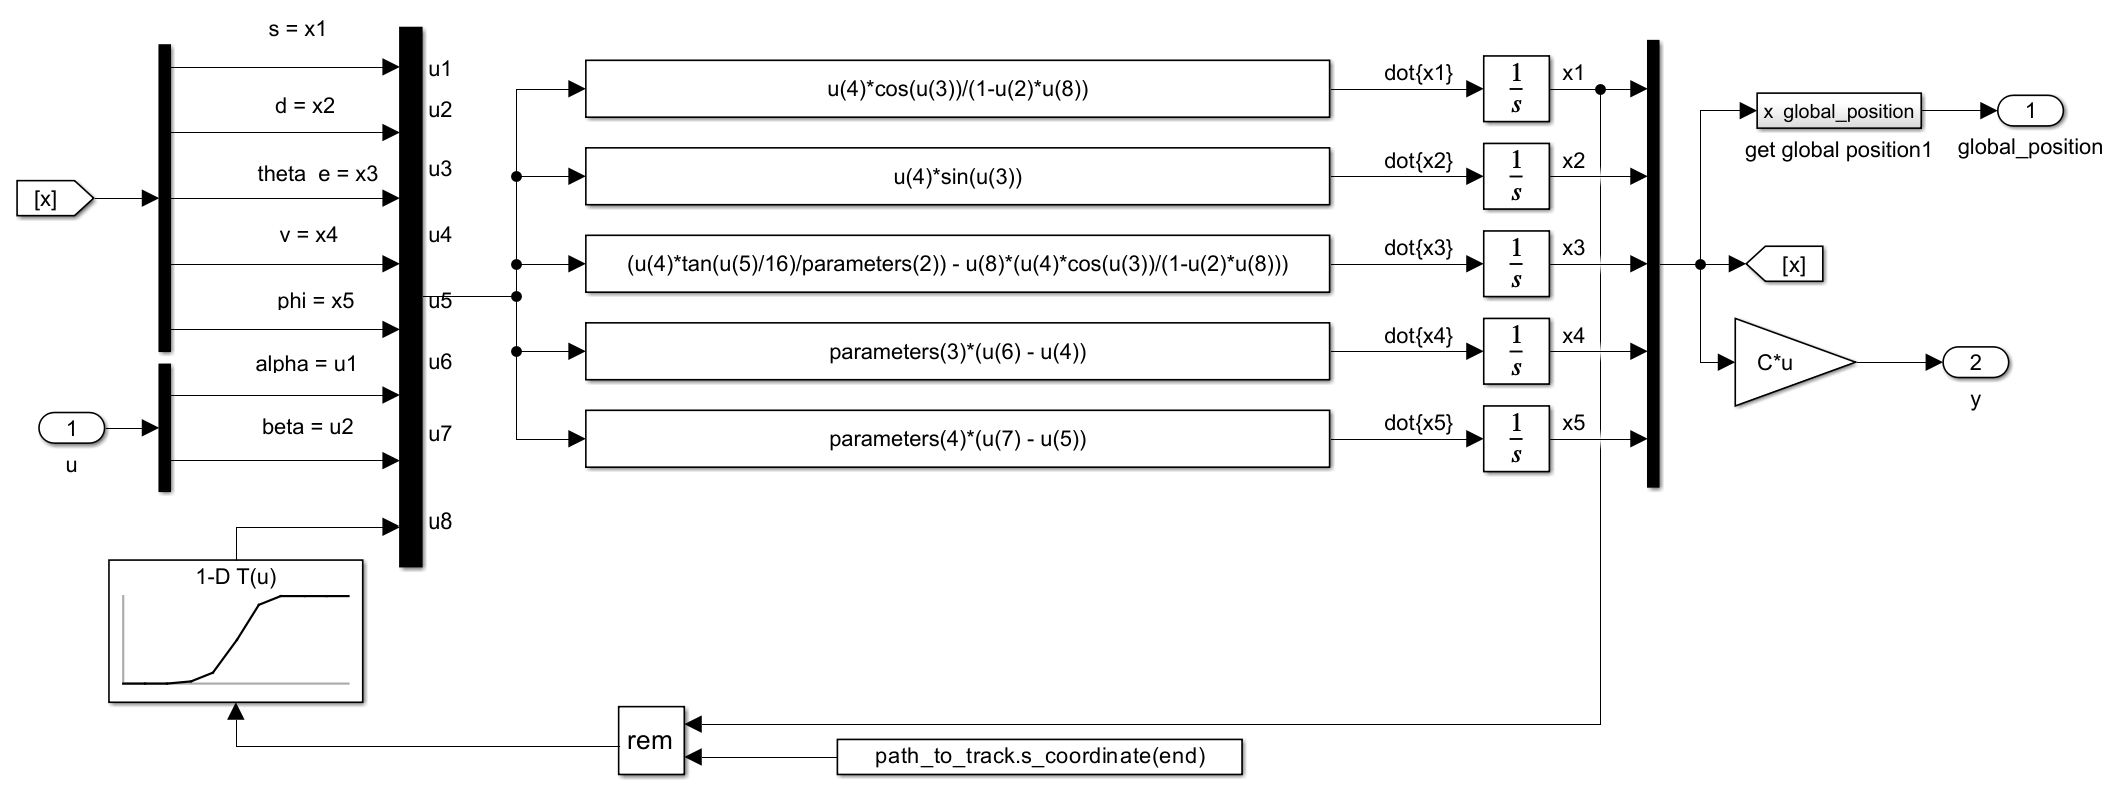
\includegraphics[width = 0.9\linewidth]{Latex report/image/nonLinModelContinousTime.png}
    \caption{Non linear model in continous time implementation in Simulink}
    \label{fig:continousTimeSimulink}
\end{figure}




\subsection{Provide a screenshot of the block diagram implemented in open loop experiments.slx.}
\begin{figure}[H]
    \centering
    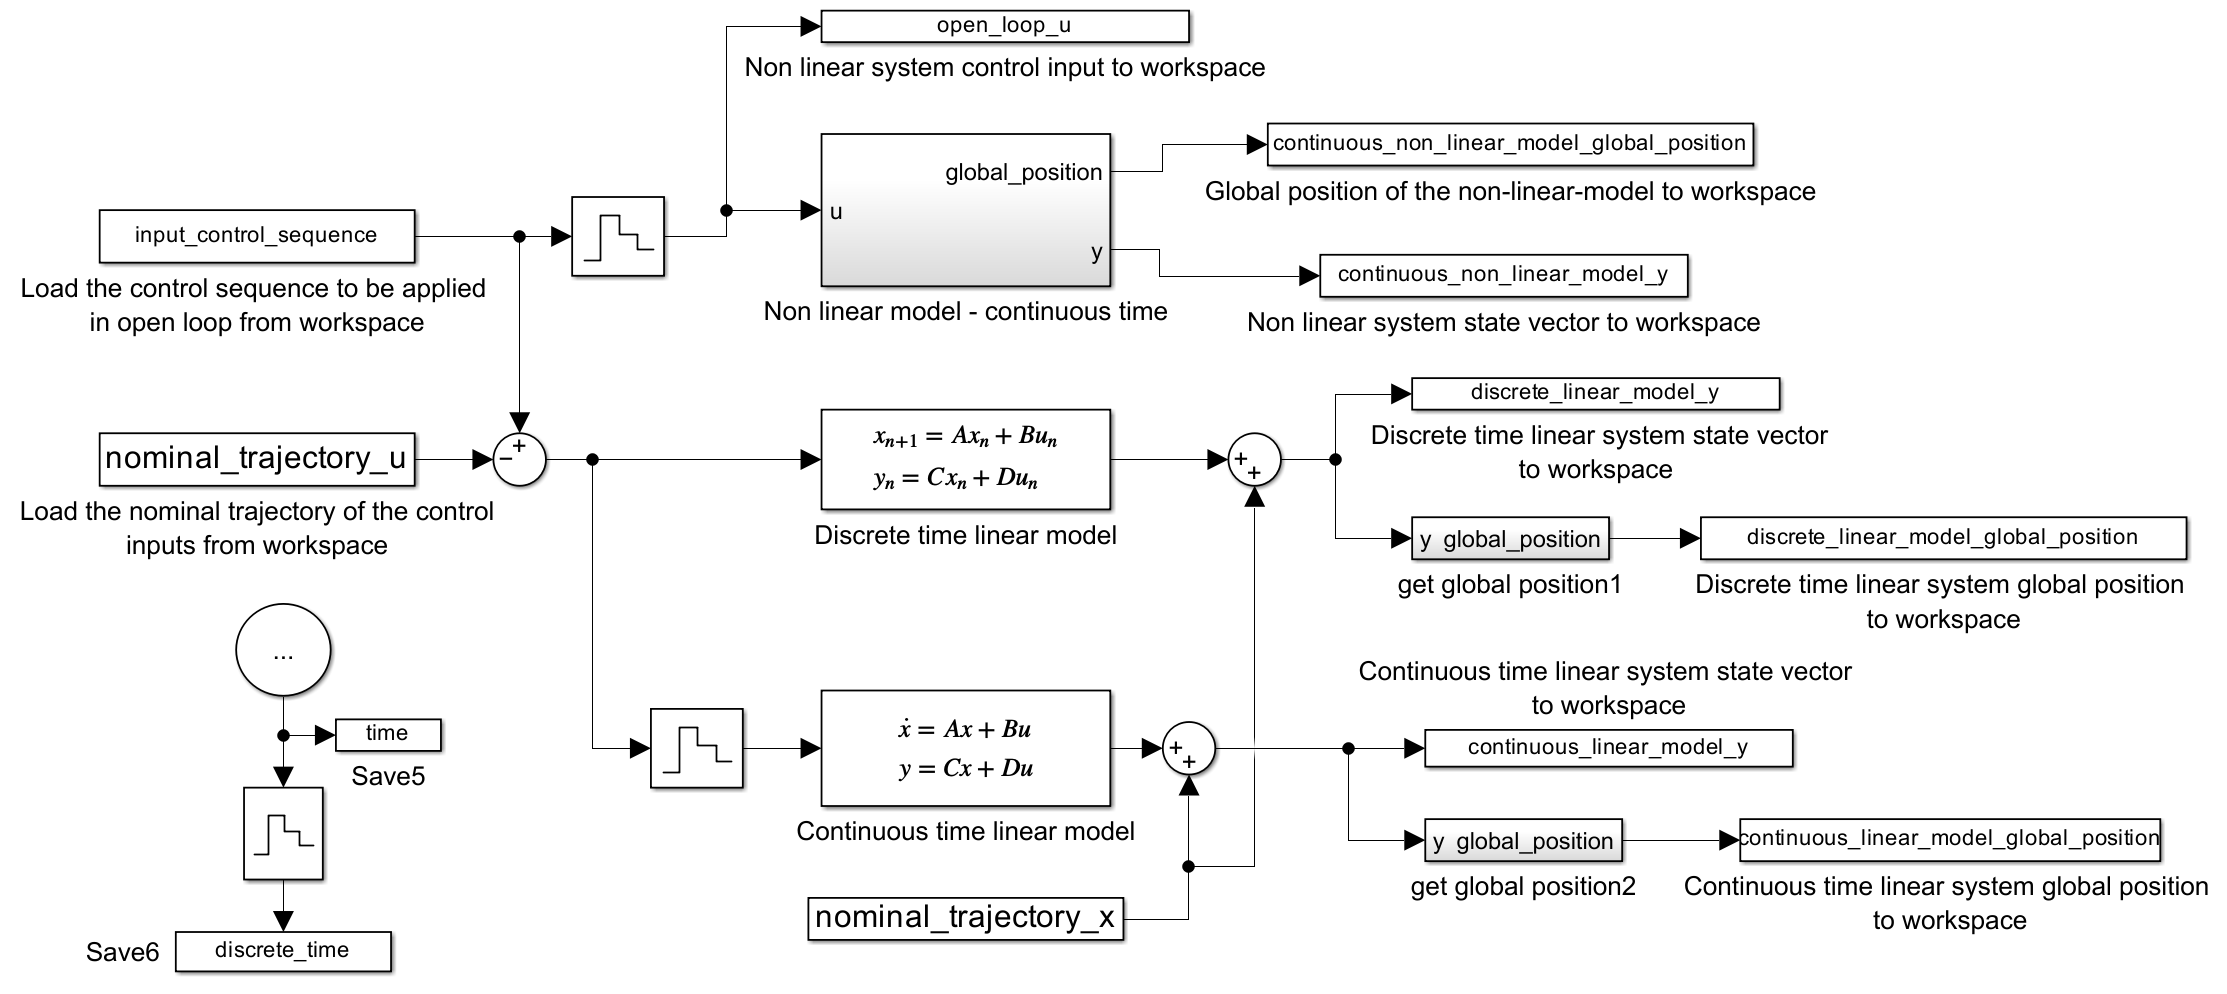
\includegraphics[width = 0.9\linewidth]{Latex report/image/ex1Simulink.png}
    \caption{Simulink diagram of exercise 1}
    \label{fig:simulinkEx1}
\end{figure}





\subsection{Report the simulation results, including the information concerning the initial state you used, the sequence of inputs you applied, and the simulated results.}

Two experiments were designed to illustrate the divergence or not of the different models developed previously. For this purpose two input sequences were constructed. The vehicle moves at a constant speed $v_{ref}$, but the steering wheel reference follows a sine function of two periods over the simulation time. It is the amplitude of this sine that will vary between the two experiments. They have been displayed side by side at the same scale in Figure \ref{fig:inputEx1}.

Experiment 1 was designed to highlight the discrepancies between the non-linear model and the two linear models. Indeed, the latter have been linearized around a point (thanks to the small signals model) and when we deviate too much from this point the approximation is no longer valid and divergences between the models appear. 
On the other hand, as for experiment 2, as long as we limit ourselves to small deviations around the linearisation point, the approximation is reasonable and we do not observe any notable differences between the results of the different models


\begin{figure}[H]
    \centering
     \begin{subfigure}[b]{0.45\textwidth}
         \centering
         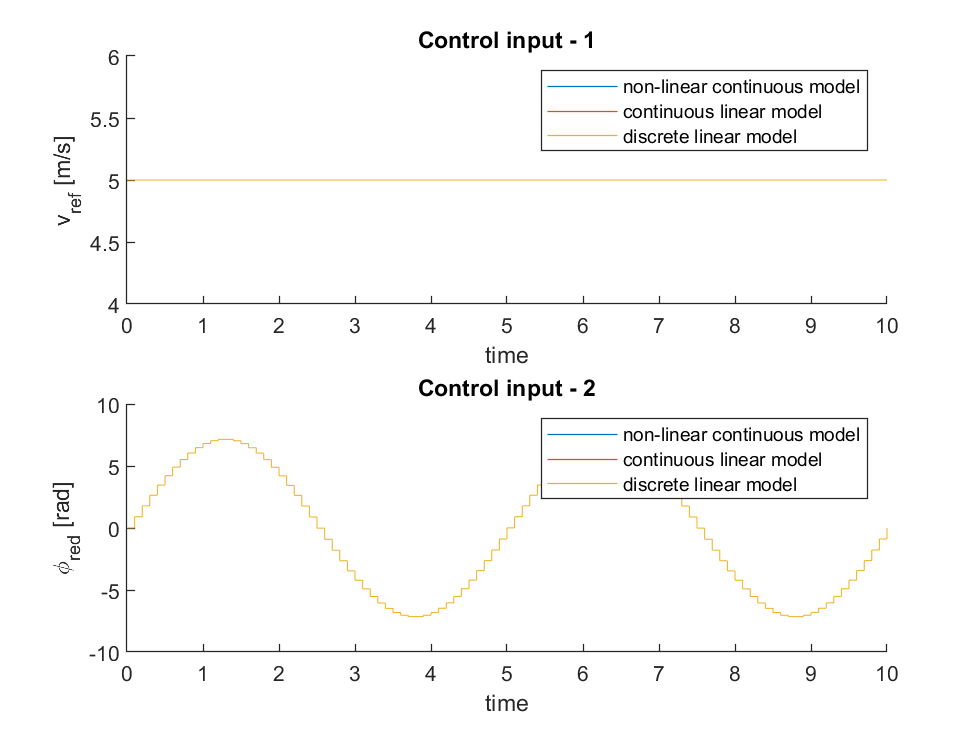
\includegraphics[width=\textwidth]{Latex report/image/ex1/input1.png}
         \caption{Input sequence 1}
         \label{fig:input11}
     \end{subfigure}
     \begin{subfigure}[b]{0.45\textwidth}
         \centering
         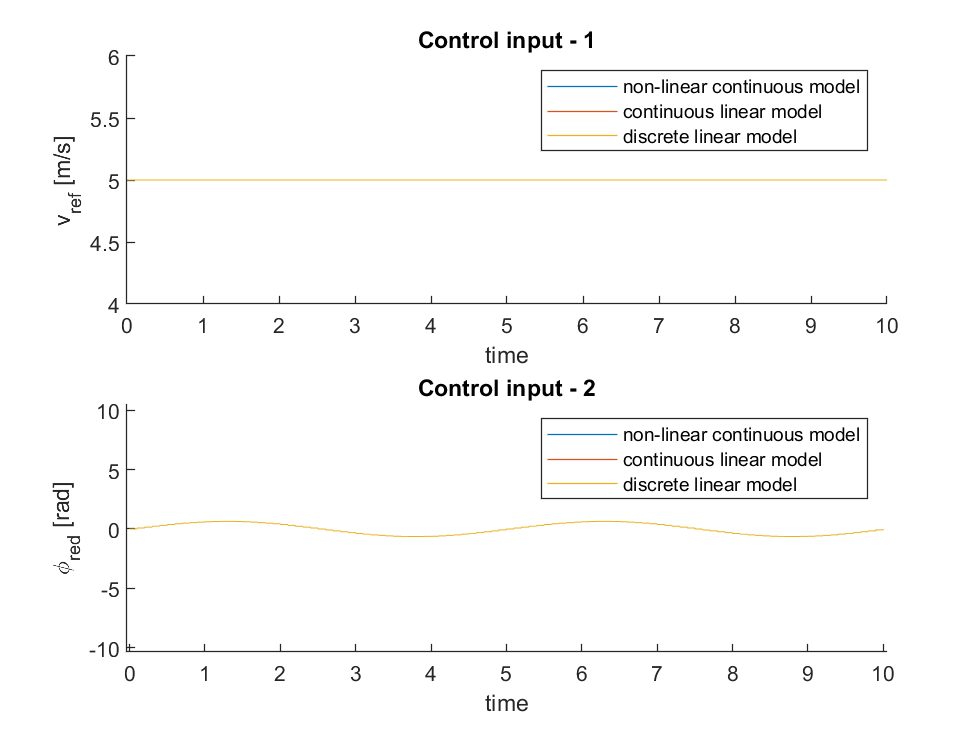
\includegraphics[width=\textwidth]{Latex report/image/ex1/input2.png}
         \caption{Input sequence 2}
         \label{fig:inpu12}
     \end{subfigure}
    \caption{Input sequence applied to the three different model used in exercise 1}
    \label{fig:inputEx1}
\end{figure}

\begin{figure}[H]
    \centering
     \begin{subfigure}[b]{0.45\textwidth}
         \centering
         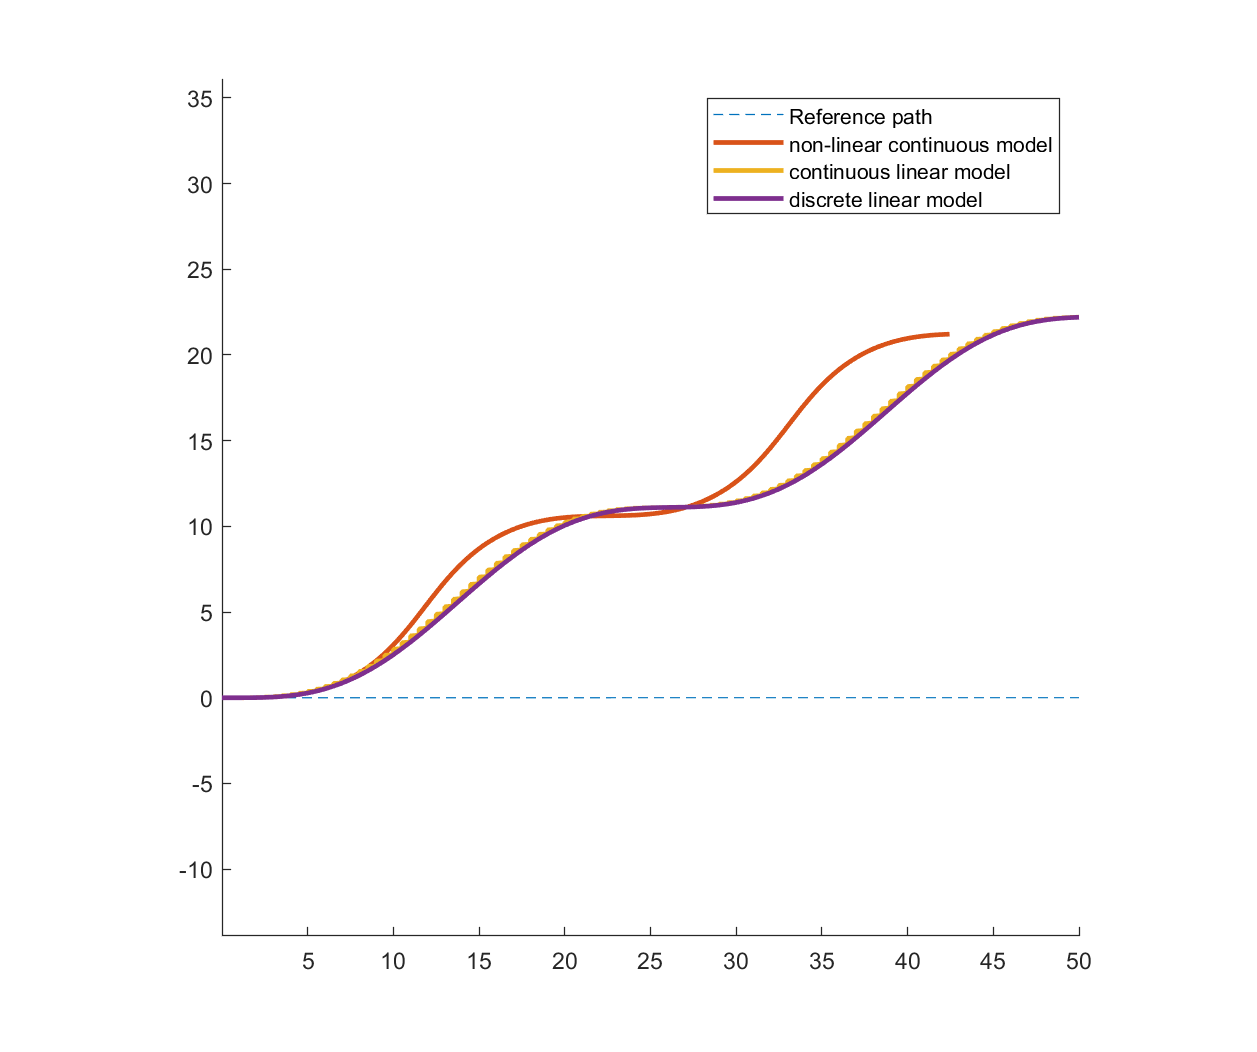
\includegraphics[width=\textwidth]{Latex report/image/ex1/trajectory1.png}
         \caption{Trajectory for experiment 1}
         \label{fig:traj11}
     \end{subfigure}
     \begin{subfigure}[b]{0.45\textwidth}
         \centering
         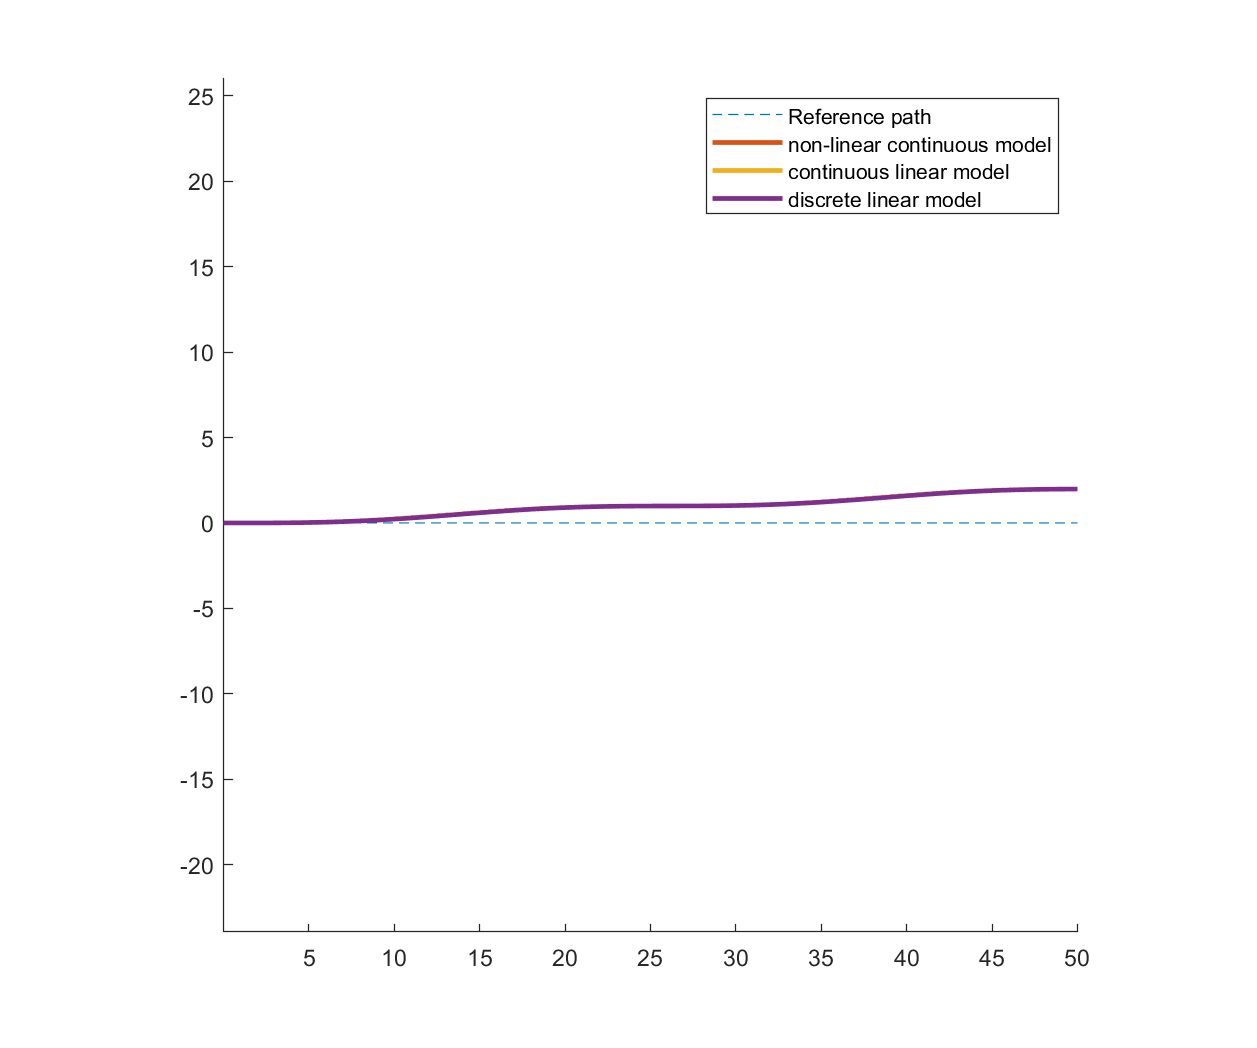
\includegraphics[width=\textwidth]{Latex report/image/ex1/trajectory2.png}
         \caption{Trajectory for experiment 2}
         \label{fig:traj12}
     \end{subfigure}
    \caption{Trajectory of the vehicle according to the three different model used in exercise 1}
    \label{fig:trajEx1}
\end{figure}

\begin{figure}[H]
    \centering
     \begin{subfigure}[b]{0.8\textwidth}
         \centering
         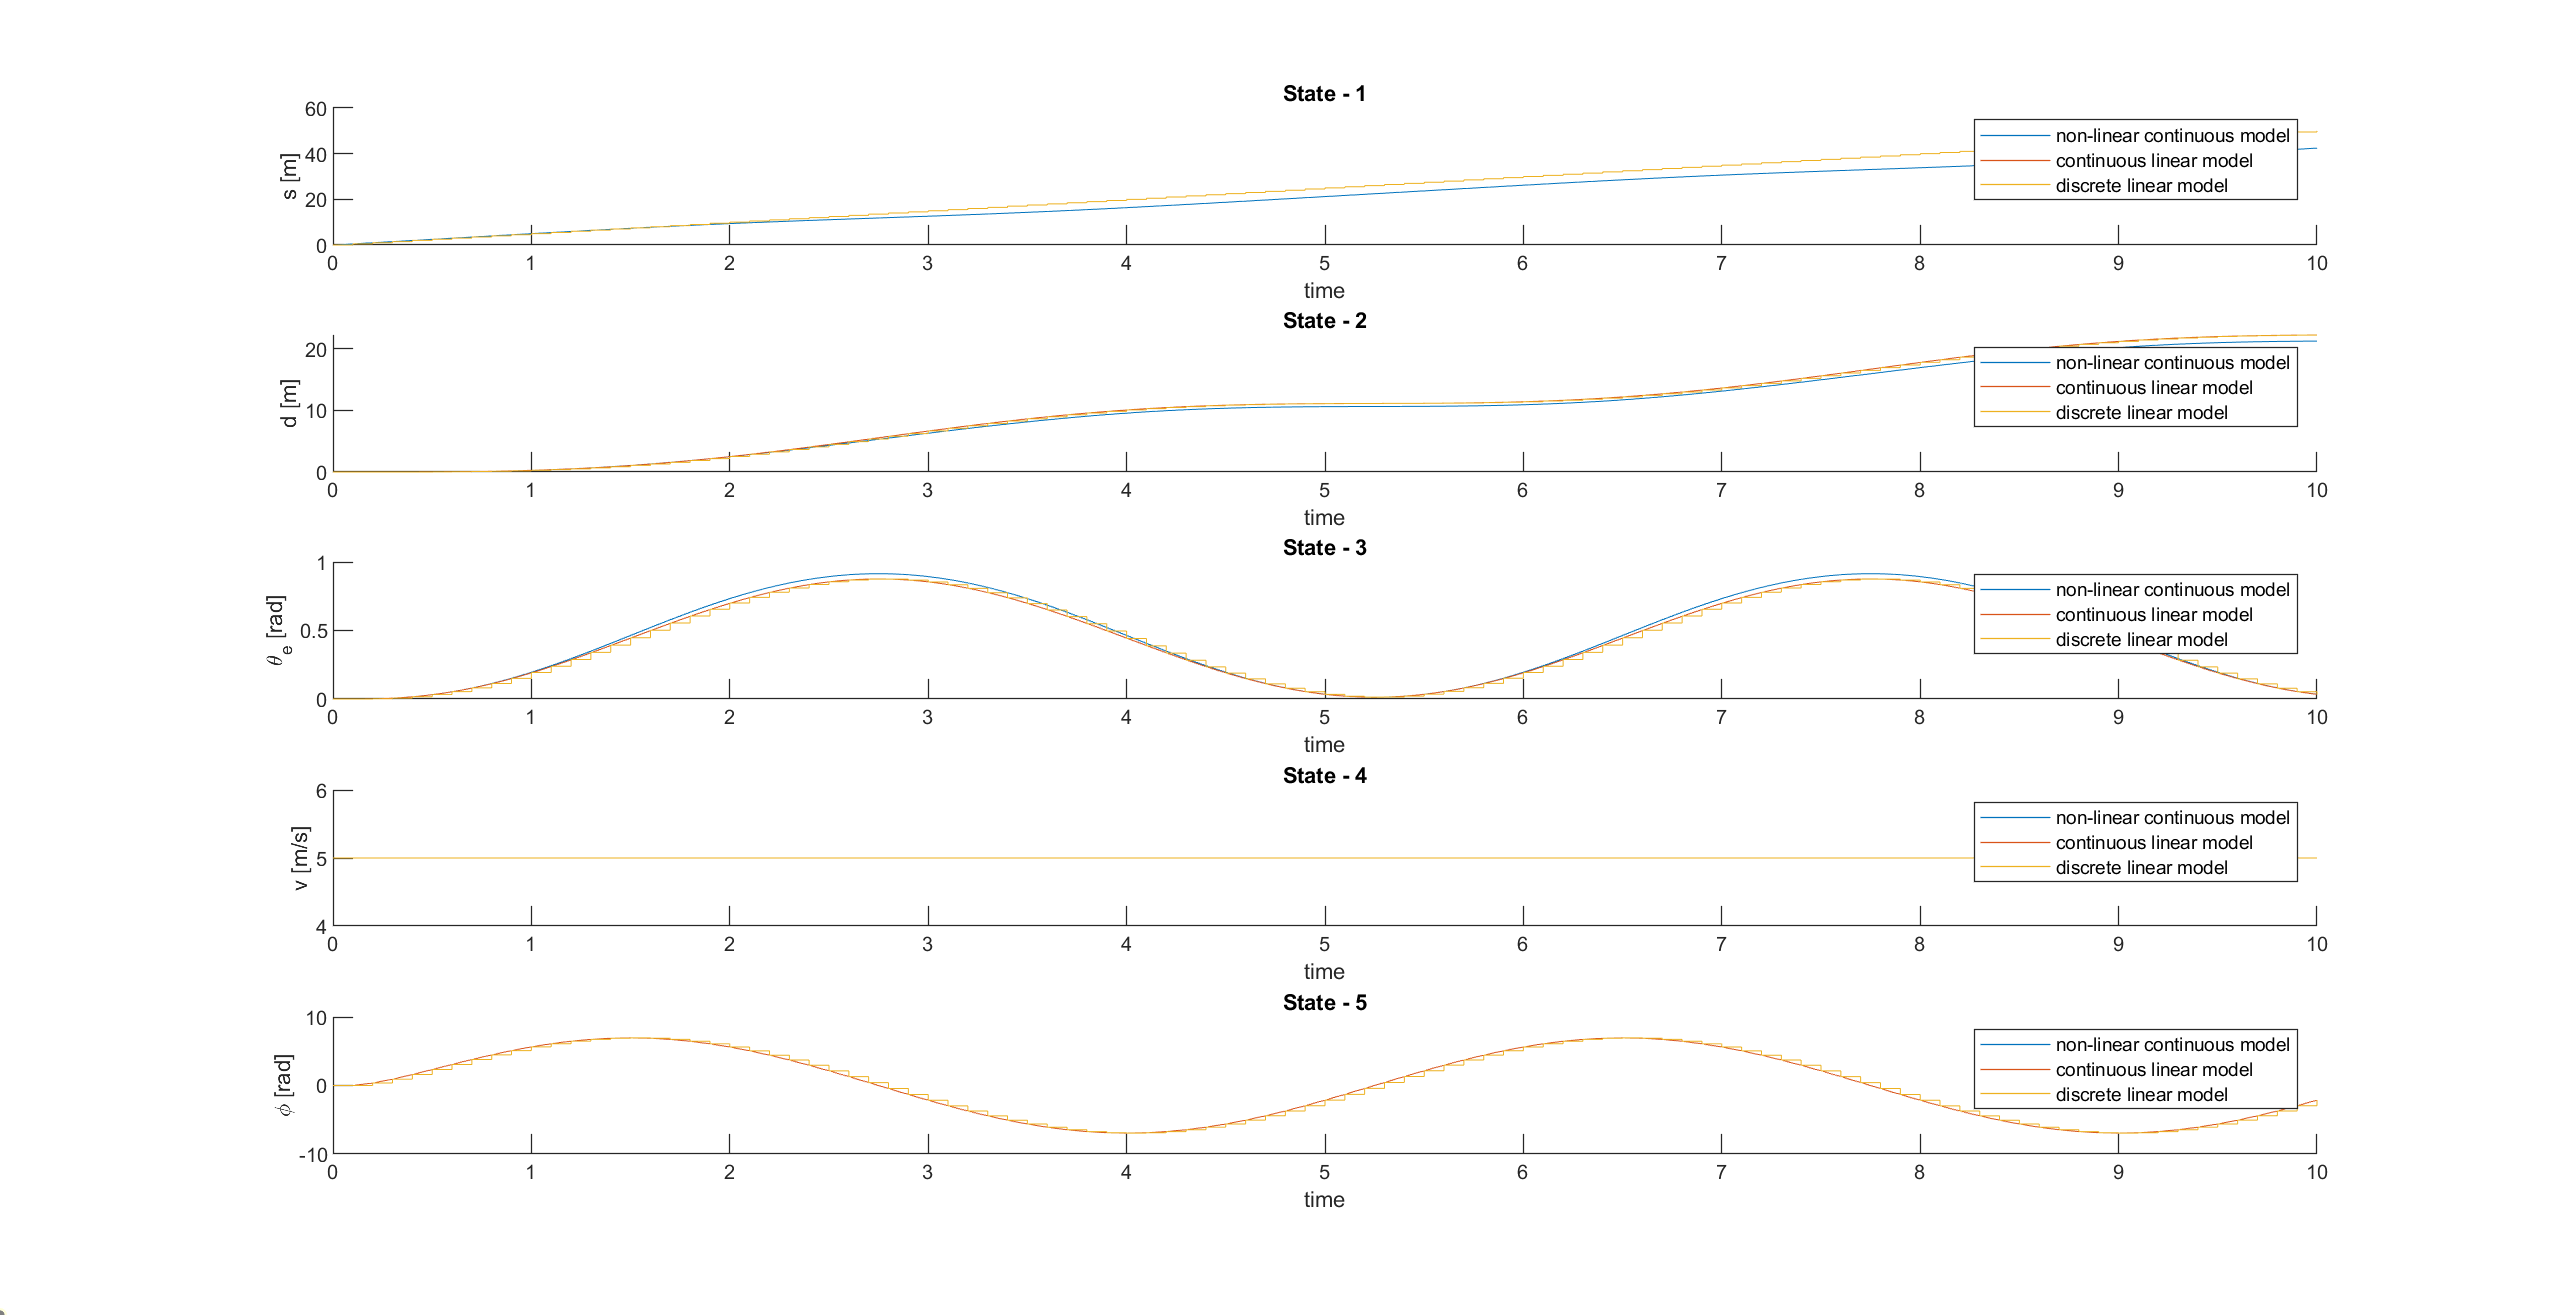
\includegraphics[width=\textwidth]{Latex report/image/ex1/state1.png}
         \caption{State for experiment 1}
         \label{fig:state11}
     \end{subfigure}
     \begin{subfigure}[b]{0.8\textwidth}
         \centering
         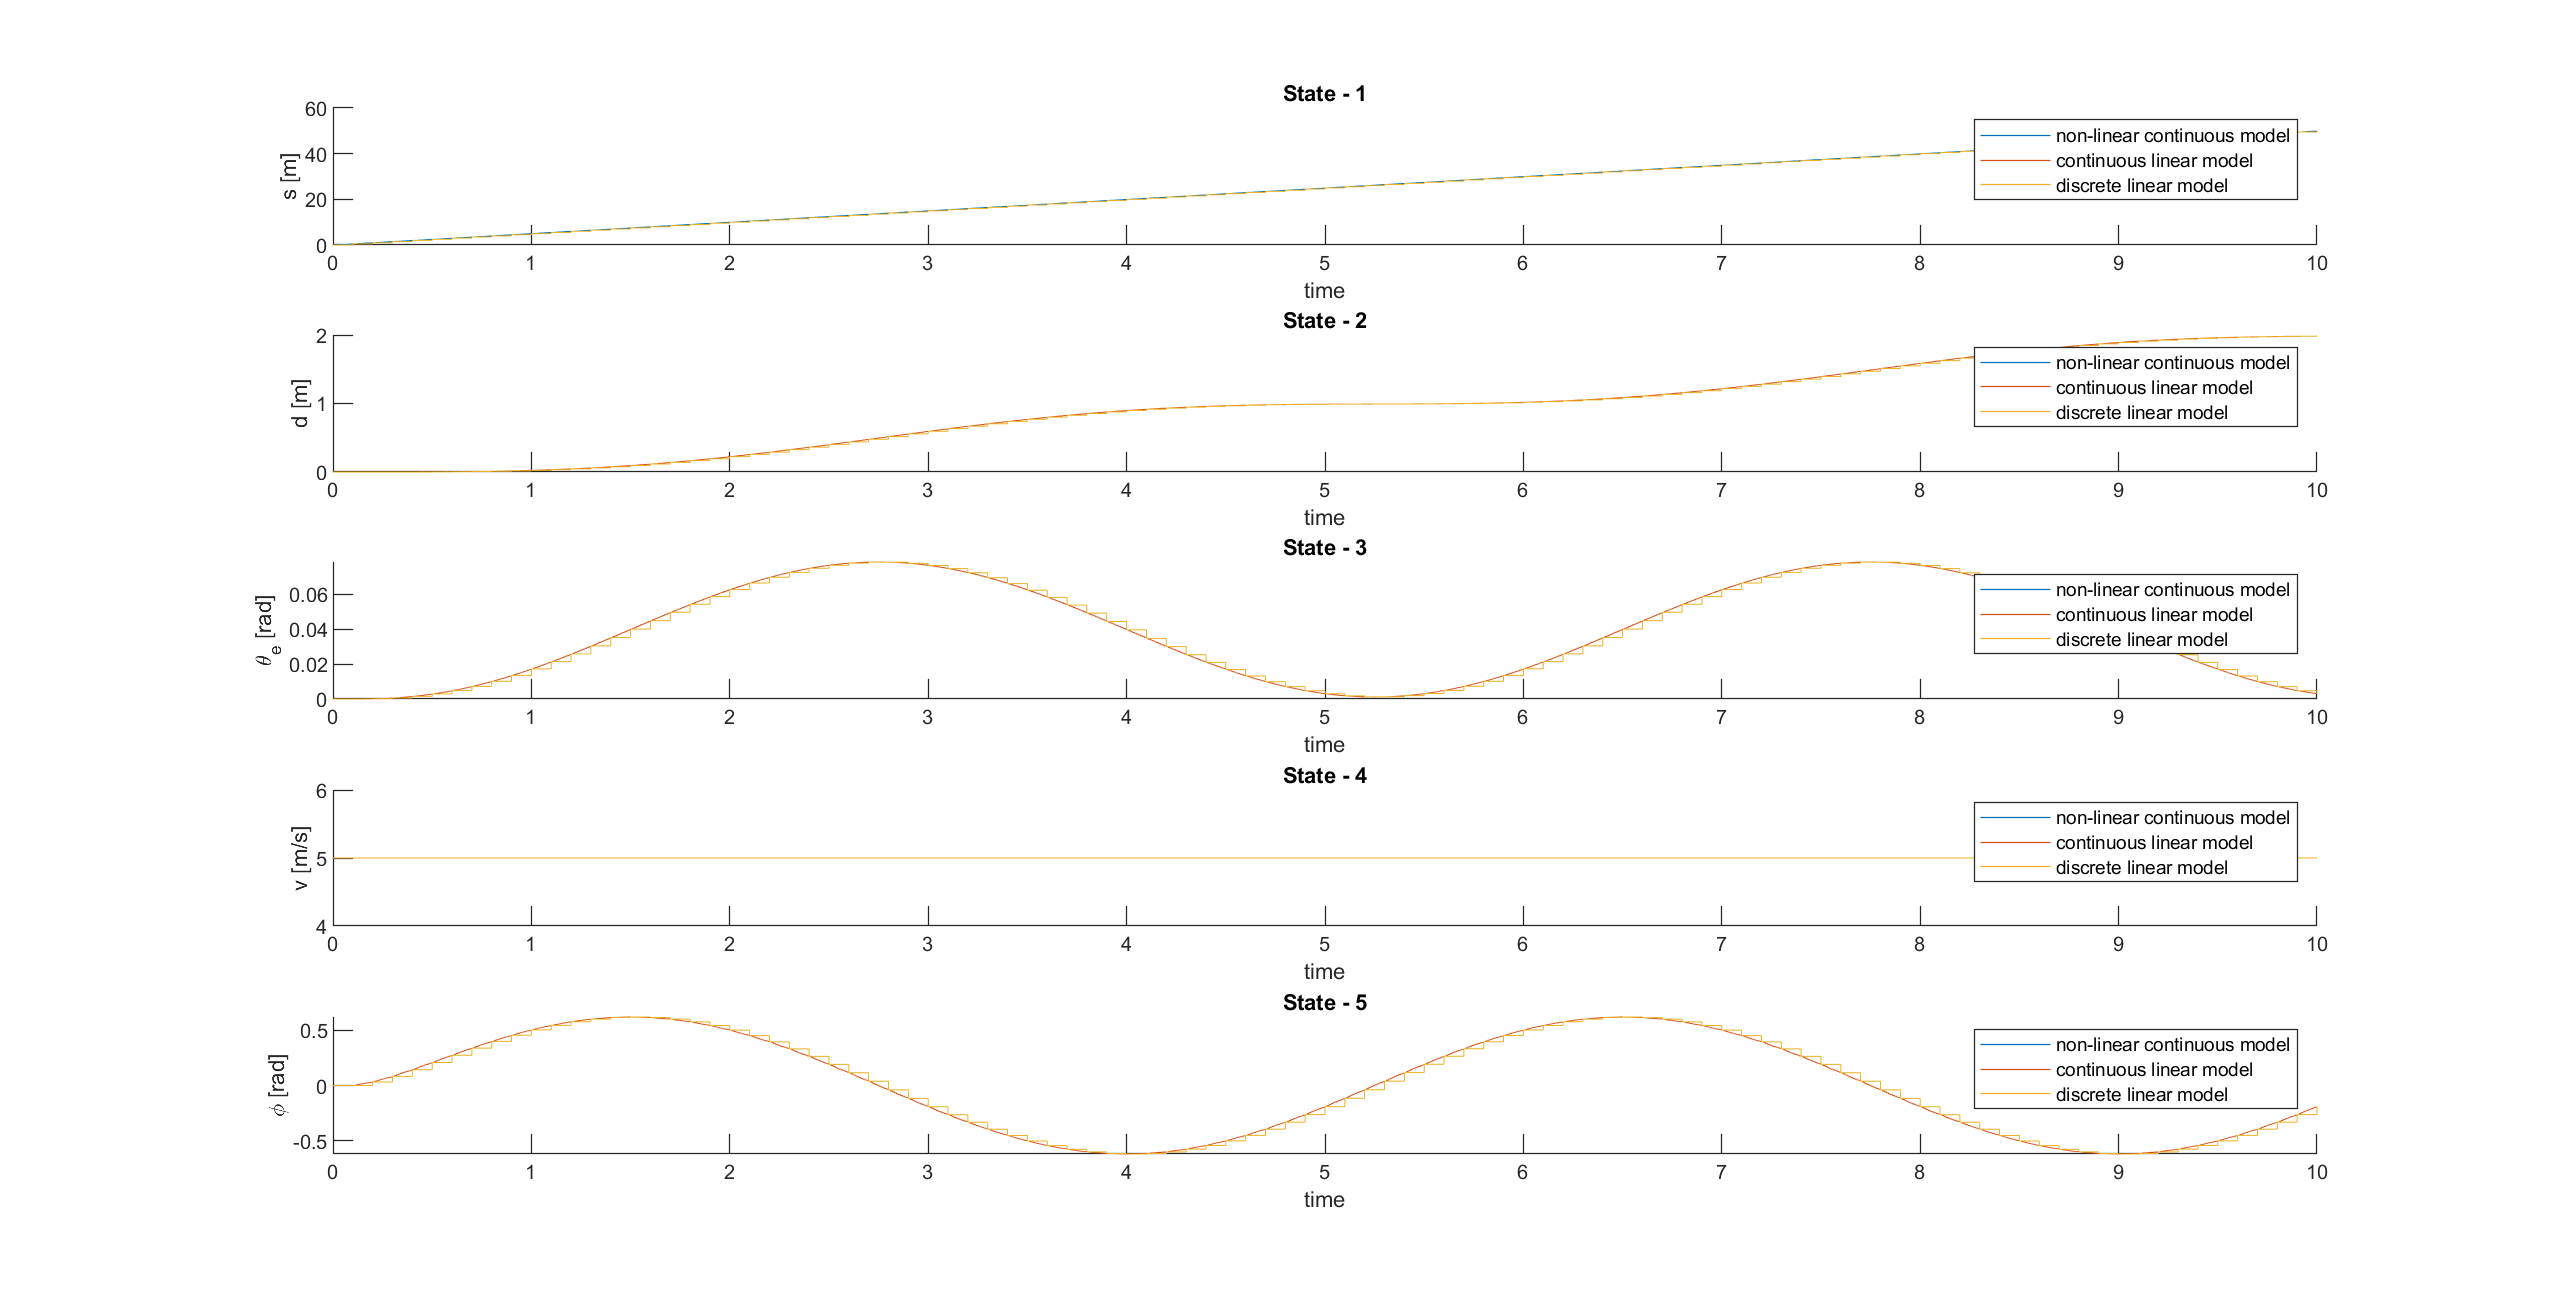
\includegraphics[width=\textwidth]{Latex report/image/ex1/state2.png}
         \caption{State for experiment 2}
         \label{fig:state12}
     \end{subfigure}
    \caption{State of the vehicle according to the three different model used in exercise 1}
    \label{fig:stateEx1}
\end{figure}



\subsection{Does the linear model resemble sufficiently well the behavior obtained from the non-linear model? Why?}

As observed, there is no simple answer to this question. Indeed, as long as one remains close enough to the linearisation point, the linear model performs as well as the non-linear model, and has the advantage of being much simpler. On the other hand, as soon as one moves away from the linearisation point, as in experiment 1, the linear model gives different results.

The differences between the linear and non-linear model can be explained by the error term (the reminder) associated with the Taylor expansion used for the linearisation. The reminder of the first order can be written in Lagrangian form \cite{Taylor}:
\begin{equation}
    R_1(x) = \frac{f^{(2)}(\zeta}{2!}(x-a)^2
\end{equation}
\\
It can be seen from the above formula that the errors between the models come from the second or higher order components of the function being linearized.

If we take the non-linear model $f(x)$, we see that $f_1(x)$, $f_2(x)$ and $f_3(x)$ contain them (with the functions sin, cos and tan), while $f_4(x)$ and $f_5(x)$ do not. This is consistent with the observations that can be made. Indeed, the states $x_1$, $x_2$ and $x_3$ diverge between the models, while the states $x_4$ and $x_5$ remains the same.\\

To conclude, the linear model is good as long as it remains close to the linearisation point, but as seen, if the vehicle moves away from it, it is no longer the case. In context of steering an an automated vehicle, susceptible of making a circle, the linear model (as it is) will not be sufficient.


\subsection{Do the results obtained using the discrete-time linear model resemble those obtained by the continuous-time linear model? What is then interesting about using the discrete-time linear model instead of the continuous-time linear model to design control strategies?}

In the two experiments presented above, the discrete time and continuous time models give very similar results. 
The discrete time model has the advantage that it corresponds to what a computer can compute in a digital world. Furthermore, it is much less computationally intensive, and can therefore be much more easily implemented in a vehicle, where space and energy are limited.



